\section{The Landscape of Rationality for Relations over Finite Words}
\label{sec:preliminaries-automatic-structures-relations}

\subsection{Regularity is Key...}

The class of "regular languages" is remarkably stable, and can either be characterized as the 
languages recognized by either:
\begin{itemize}
	\item deterministic or non-deterministic finite state automata,\\
		\null\hspace{1.0pc}see "eg" \cite[Proposition~1.2.3, p.~7]{Pin2021FiniteAutomata};
	\item two-way finite state automata by Shepherdson-Rabin-Scott theorem\\
		\null\hspace{1.0pc}\cite[Theorem~2, p.~198]{Shepherdson1959ReductionTwoWay}
		\cite[Theorem~15, p.~123]{RabinScott1959FiniteAutomata};
	\item rational expressions by Kleene's theorem,\\
		\null\hspace{1.0pc}see "eg" \cite[Theorem~1.5.11, p.~34]{Pin2021FiniteAutomata};
	\item monadic second-order logic by Trakhtenbrot-Büchi-Elgot theorem,\\
		\null\hspace{1.0pc}see "eg" \cite[Theorem~2.2, p.~32]{Bojanczyk2020MSO}; or
	\item finite monoids, see "eg" \cite[\S~1.4.2, p.~19]{Pin2021FiniteAutomata}.
\end{itemize}
Moreover, all transformations between these representations are effective---although some
models can be strictly more succinct.

\begin{figure*}
	\centering
	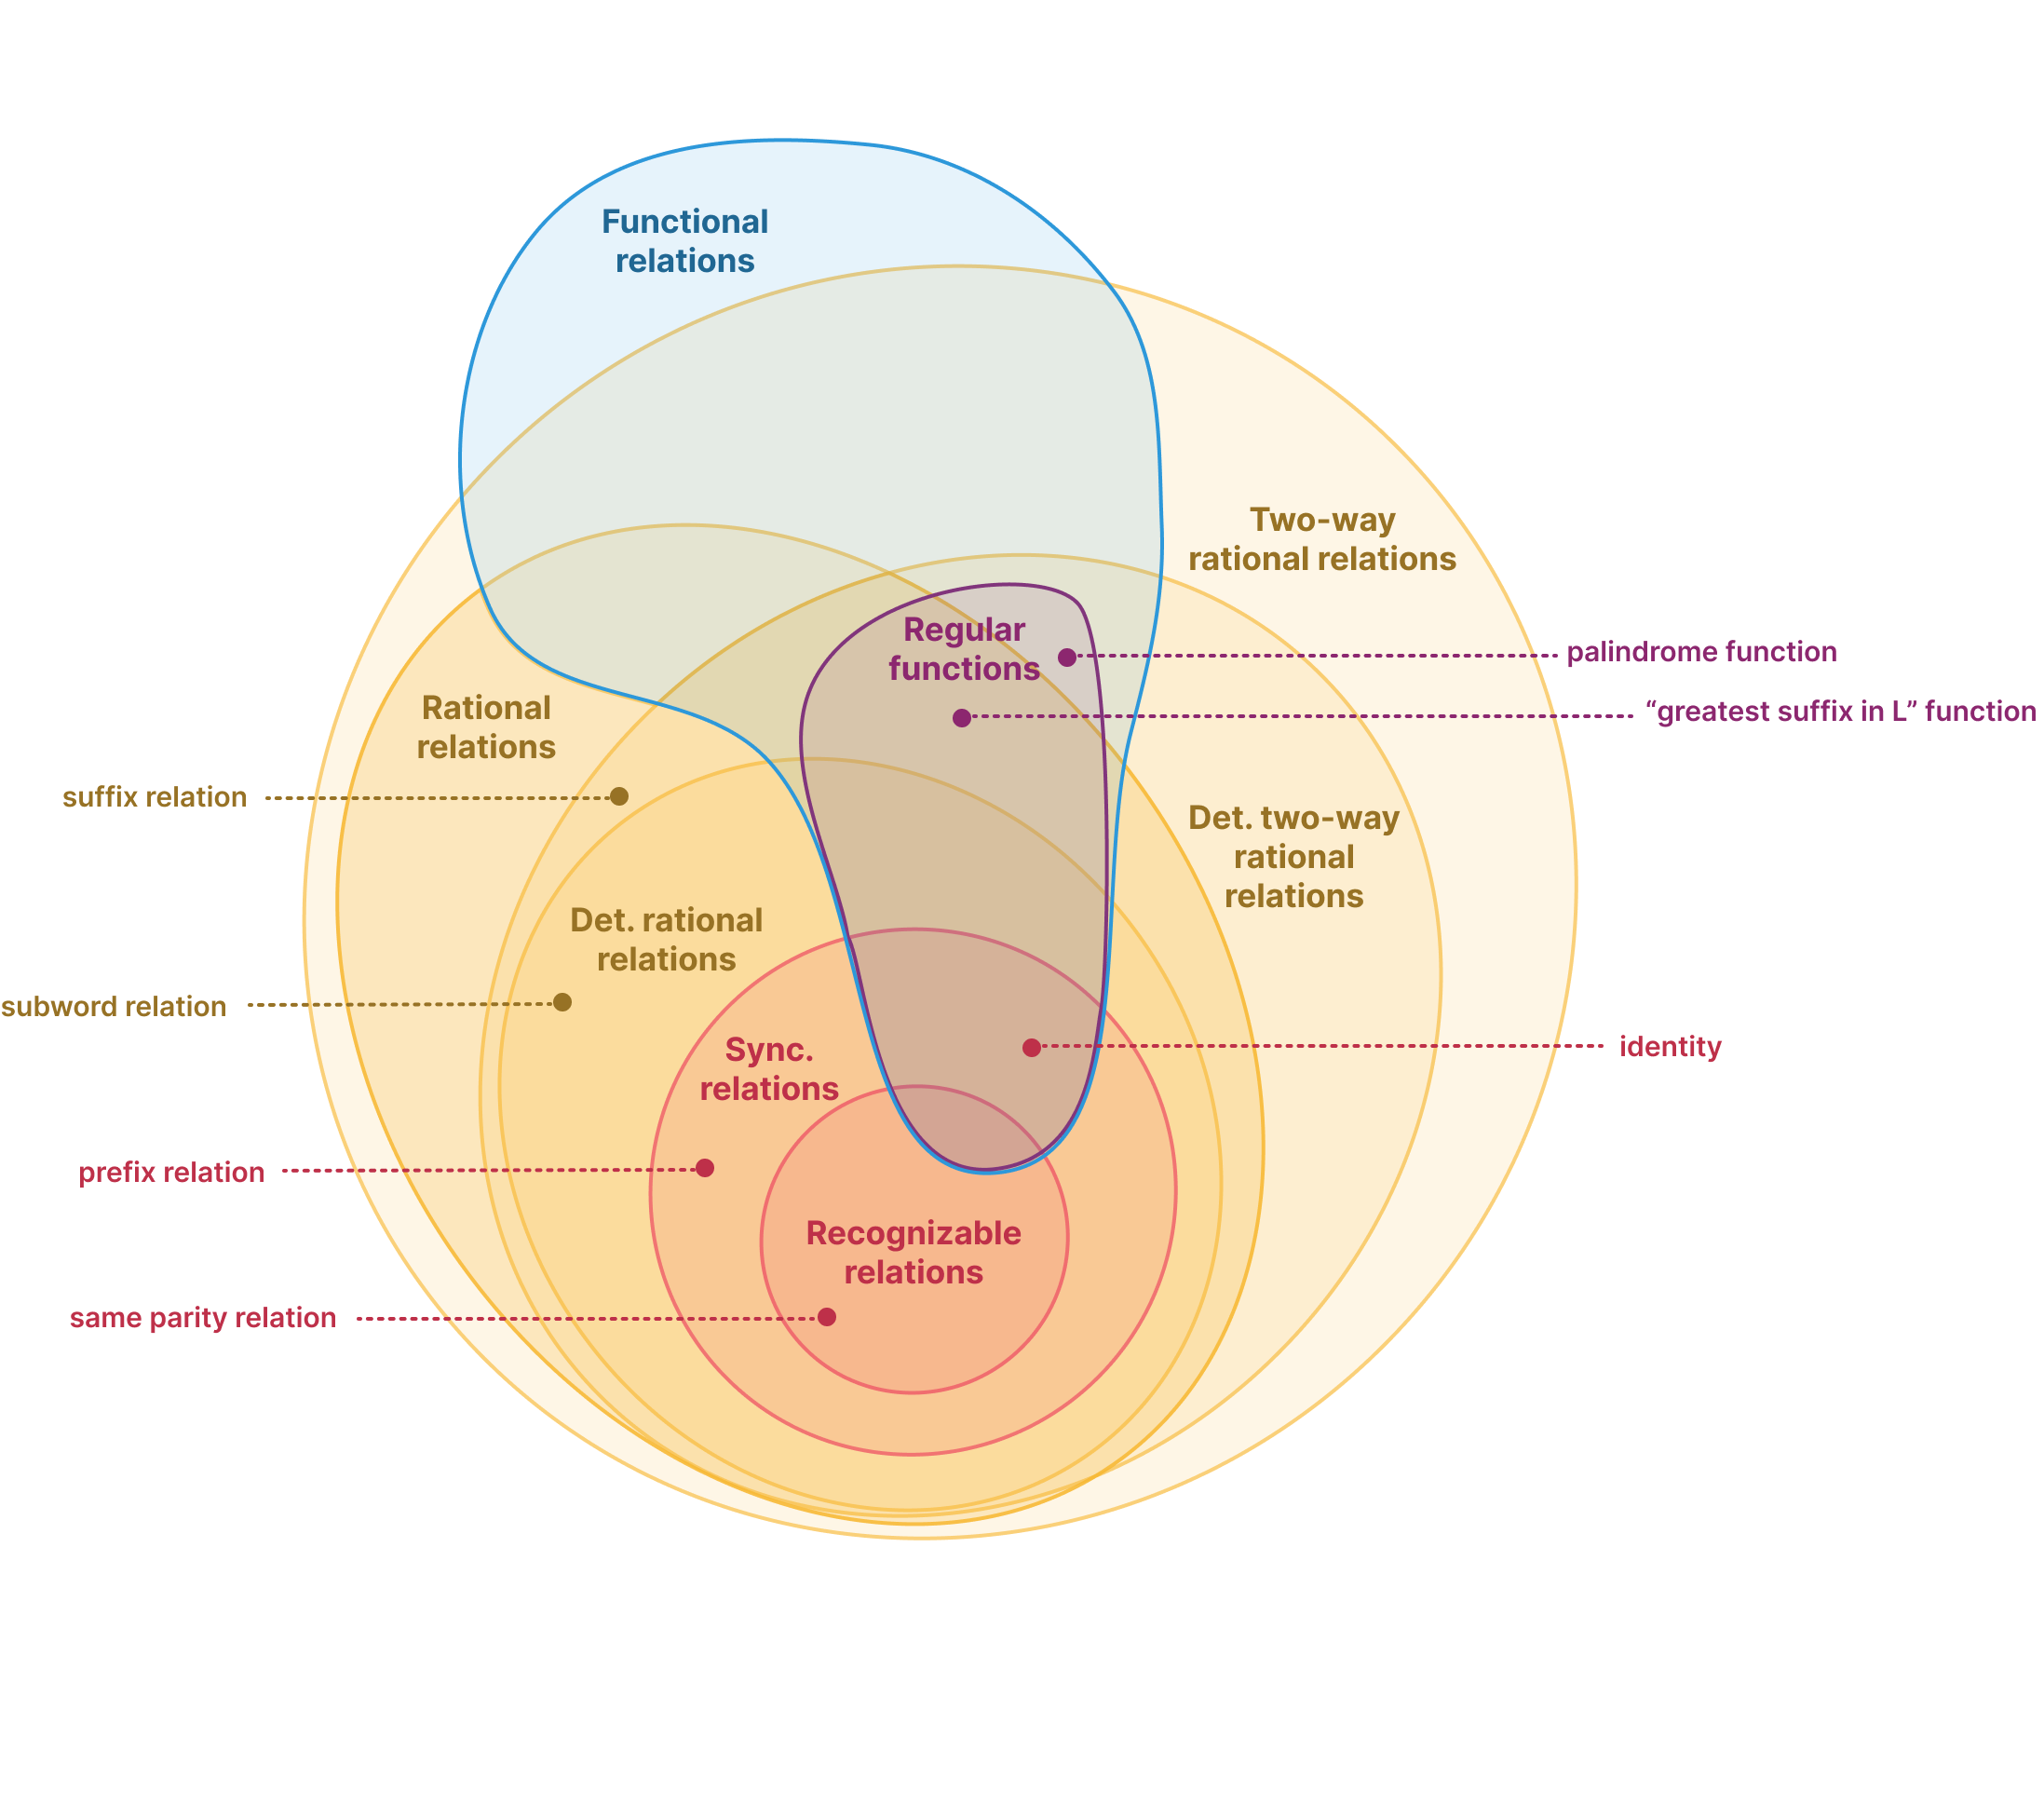
\includegraphics[width=\linewidth]{fig/landscape-rationality-relations.png}
	\caption{
		\AP\label{fig:landscape-rationality-relations}
		The ``landscape of rationality'' for binary relations.
		Dashed regions are empty.
		TODO:UPDATE: SUFFIX RELATION IS Deterministic TWO-WAY AND RATIONAL.
	}
\end{figure*}
These equivalences explain why the terms \emph{recognizable language}---meaning implicitly
``recognizable by a finite-state automaton'' or ``recognizable by a finite monoid''---and
\emph{rational language}---meaning ``described by a rational expression''---are used 
interchangeably. In fact, in this thesis as well as in most of the literature,
we will use the generic term "regular language".
However, in more complex settings, for instance subsets of non-free monoids,%
\footnote{Recall that a language is nothing else but a subset of a free
(usually finitely-generated) monoid.}
the equivalence between these classes no longer holds. \cite{Pin2021StackExchange}

The landscape of rationality for $k$-ary relations of finite words ($k \geq 2$) is far more complex than for languages,\footnote{Which can be seen as unary relations of finite words.} as depicted in \Cref{fig:landscape-rationality-relations}. We will briefly present these classes,
although this thesis will only deal with the two most restrictive ones, namely
"recognizable@@rel" and "automatic relations".%
\footnote{It should be noted that the names
of these classes were often coined independently of one another---sometimes defying common sense.
For instance, "automatic relations" are named this way because they correspond to
the relations recognized by some model of automata...
not unlike most of the classes in \Cref{fig:landscape-rationality-relations}.
They are also sometimes named ``regular relations'', which have nothing to do
with "regular functions" and do \emph{not} correspond to the intersection of "regular functions"
with "functional relations", as one would reasonably expect.}
We fix two alphabets $\Gamma$ and $\Sigma$. In the rest of this section, we focus
on relations $\+R \subseteq \Gamma^* \times \Sigma^*$, "aka" transductions.

\paragraph*{Goal of this section.}
When I learned about these classes, I was somewhat confused between the different models: surprisingly, the literature on transductions seems somewhat orthogonal to the one on relation.%
\footnote{For instance \cite{Choffrut2006Survey} mentions todo, but not todo. On the other hand todo.}
The goal of this section is to provide a non-exhaustive overview of these classes of relations/transductions, explain how they relate to one another, and give pointers to suitable references.
We acknowledge \cite{Choffrut2006Survey}, which proved particularly useful to find the
appropriate references. Of course, the aim of this section is not to be exhaustive,
which would be a daunting task,%
\footnote{Sakarovitch's book \cite{Sakarovitch2009Elements}
dedicates its second part to ``Rationality in relations'', which spans over more than two hundred pages---one can only imagine how extensive this part could have been if the book was not
dedicated to presenting \emph{elements} of automata theory but the full theory itself!}
but rather to present a quick overview of the most common classes of relations
studied in the literature.
todo:most can be skipped.

\paragraph*{Relations "vs" transductions.}
Often, in the literature, when the terminology ``transduction'' is used,
these relations are thought as functions from $\Gamma^*$ to $\pset{\Sigma^*}$---sometimes
assuming that the input is a singleton, sometimes not---,
and in this case $\Gamma$ (resp. $\Sigma$) plays the role of an ``input alphabet''
(resp. ``output alphabet''). A transducer reads a letter from the input alphabet,
and \emph{produces} a letter from the output alphabet: inherently, transducers are seen
as a machine that \emph{produces} an ouput, or rather that \emph{tranduces} an input into an output, or multiple outputs.

On the other hand, when the terminology ``relation'' is used,
we often take $\Gamma = \Sigma$.\footnote{For instance this is somewhat important when
dealing with logic or defining automatic structure
\Cref{sec:preliminaries-automatic-structures-automatic-structures,sec:preliminaries-automatic-structures-logic}.}
Multitape automata are seen as machine that read
tuples of words, and either accept or reject them: it is a decision model.
The question of $\Gamma =^? \Sigma$ makes little difference since we can often
see a relation $\+R \subseteq \Gamma^* \times \Sigma^*$ as a subset of
$(\Gamma\sqcup \Sigma)^* \times (\Gamma\sqcup \Sigma)^*$
while preserving the notion of ``rationality'' at hand.
Moreover, we will see that some classes can be equally defined
by using multitape automata or transducers todo:addref.

Note also that most notions defined by multitape automata
can be trivially extended to $k$-ary relations ($k \geq 3$):
we simply work here with binary relations for the sake of simplicity---we will sometimes give more general definition for higher arity when the generalization is not trivial.
On the other hand, transducers intrinsically recognize functions $\Gamma^* \to \pset{\Sigma^*}$,
"ie" binary relations.

Given two classes of finite-word relations $\+C$ and $\+D$ "st" $\+C \supseteq \+D$,
we will often want to know if this inclusion is \emph{effective}:
\decisionproblem{
	""$\+D$-membership problem for $\+C$-relations""
}{
	A $\+C$-relation $\+R$.
}{
	Does $\+R \in \+D$?
}
This problem is also called the \reintro{$\+C$/$\+D$-membership problem}.

A natural extension of this problem is the so-called separability problem,
which has received lots of attention in todo:addref.
\decisionproblem{
	""$\+D$-separability problem for $\+C$-relations""
}{
	Two $\+C$-relations $\+R$ and $\+R'$.
}{
	Is there a $\+D$-relation "st" $\+R \subseteq \+S$ and $\+R' \cap \+S = \emptyset$?
}
In this case, we say that $\+S$ ""separates@@rel"" $\+R$ from $\+R'$.
Note that when $\+D$ is closed under complement, $\+R$ and $\+R'$ play a symmetric role in this problem. Moreover, if $\+D$ is \emph{effectively} closed under complement,
then "membership@@problemrel" reduces to "separability@@problemrel" 
since $\+R in \+D$ if, and only if, $\+R$ and its complement are "separable@@rel" by
a $\+D$-relation.


\subsection{Recognizable Relations}

A relation $\+R \subseteq \Gamma^* \times \Sigma^*$ is \AP""recognizable@@rel""
if there exists a "finite monoid" $\?M$ together with a "monoid morphism"
\[
	f\colon \Gamma^* \times \Sigma^* \to \?M,
\]
as well as a subset $\Acc \subseteq M$ "st"
$\+R = f^{-1}[\Acc]$. We denote by \AP$\intro*\REC$ the class of "recognizable relations".%
\footnote{todo: Again, insert some set-theoretic bullshit.}

For instance the \AP""same parity relation""
\[
	{\intro*\sameParity} \defeq 
	\{
		\tup{u,v} \in \Gamma^* \times \Sigma^* \mid
		|u| = |v| \mod{2}
	\}
\]
is "recognizable@@rel". Indeed, letting $f\colon  \Gamma^* \times \Sigma^* \to \ZnZ{2}$,
then $\sameParity$ can be written as $f^{-1}[\{\bar 0\}]$.

These relations admit a remarkably simple characterization.\AP
\begin{proposition}[{""Mezei theorem"", see "eg" \cite[Corollary~II.2.20, p.~254]{Sakarovitch2009Elements}}]
	\!\footnote{\cite[\S~2, ``Notes \& references'']{Sakarovitch2009Elements} mentions
	that this proposition is ``unanimously ascribed to G. Mezei (unpublished)''.}
	\label{prop:Mezei-theorem}
	A relation $\+R$ is "recognizable@@rel" "iff" there exists $n\in\N$,
	"regular languages" $\tup{K_i}_{i\in \lBrack 1,n\rBrack}$ over $\Gamma$
	and "regular languages" $\tup{L_i}_{i\in \lBrack 1,n\rBrack}$ over $\Sigma$
	"st"
	\[
		\+R = \bigcup_{i=1}^n K_i \times L_i.
	\]
\end{proposition}

In other words, "recognizable relations" are exactly the finite unions of
"Cartesian products" of "regular languages".
For instance, \[{\sameParity} =
(\Gamma\Gamma)^* \times (\Sigma\Sigma)^*
\cup \Gamma(\Gamma\Gamma)^* \times \Sigma(\Sigma\Sigma)^*.\]
We provide a slightly more general statement of "Mezei theorem".

\begin{proposition}
	\label{prop:Mezei-theorem-generalization}
	Let $\B{V}$ be a "pseudovariety of finite monoids"
	and $\+V$ be the corresponding "pseudovariety of regular languages".
	Let $\+R \subseteq \Gamma^* \times \Sigma^*$ be a relation.
	The following are equivalent:
	\begin{enumerate}
		\item there exists a "finite monoid" $\?M \in \B{V}$, a "monoid morphism"
		$f\colon \Gamma^* \times \Sigma^* \to \?M$ and $\Acc \subseteq \?M$
		"st" $\+R = f^{-1}[\Acc]$;
		\item there exists $n \in \N$
		and $K_1,\hdots,K_n \in \+V_{\Gamma}$ and $L_1,\hdots,L_n \in \+V_{\Sigma}$
		"st" $\mathcal{R} = \bigcup_{i=1}^n K_i \times L_i$,
	\end{enumerate}
	in which case we say that $\+R$ is \AP""$\+V$-recognizable@@rel"".
\end{proposition}

When $\B{V}$ is the "pseudovariety@@reglang" of all "regular languages",
we get back \Cref{prop:Mezei-theorem}.

\begin{proof}
	\proofcase{From monoids to products.}
	Assume that $\+R$ is "recognizable@@rel". 
	Then by definition
	\[
		\+R = \bigcup_{z \in \Acc} f^{-1}[z].
	\]
	Observe then that $f(u,v) = f(\tup{u,\varepsilon}\cdot\tup{\varepsilon,v})
	= f(u,\varepsilon)\cdot f(\varepsilon,v)$ for all $u,v \in \Gamma^* \times \Sigma^*$, and hence:
	\[
		\+R = \bigcup_{\substack{x,y \in M\\ \text{"st" } x\cdot y \in \Acc}}
		\underbrace{\{u \in \Gamma^* \mid f(u, \varepsilon) = x\}}_{\defeq \;K_x}
		\times \underbrace{\{v \in \Sigma^* \mid f(\varepsilon, v) = y\}}_{\defeq \;L_y}.
	\]
	Since $M$ is finite, the union is finite, and moreover, each $K_x$ and $L_y$ is
	recognized by $M \in \B{V}$, and hence belong to $\+V$.

	\proofcase{From products to monoids.} If $\mathcal{R} = \bigcup_{i=1}^n K_i \times L_i$ 
		where all languages belong to $\+V$, then let $M_i,N_i \in \B{V}$
		be their "syntactic monoids", $g_i,h_i$ be their
		"syntactic morphism", and $\Acc_i,\Bcc_i$ be their accepting sets.
		Consider the monoid morphism
		\begin{center}
		\begin{tabular}{ccc}
			$\Gamma^* \times \Sigma^*$ & $\to$ & $\prod_{i}(M_i \times N_i)$ \\
			$\tup{u,v}$ & $\mapsto$ & $\tup{g_i(u), h_i(v)}_{i}$.
		\end{tabular}
		\end{center}
		Then $\+R$ is the preimage by this morphism of
		\[
			\bigcup_{i=1}^n \bigl(
			\cdots \times (M_{i-1}\times N_{i-1}) \times
			(\Acc_i \times \Bcc_i) \times (M_{i+1}\times N_{i+1}) \times \cdots \bigr).
		\]
		The conclusion follows from the fact that $\B{V}$ is closed under finite products.
\end{proof}

Both the algebraic definition of "recognizable relations" and
"Mezei theorem" imply---informally!---that all reasonable problems on
"recognizable relations" are decidable. For instance, from \Cref{prop:Mezei-theorem-generalization},
we get that $\+V$ has decidable "membership@@problang" "iff" the class of "$\+V$-recognizable relations"
has decidable "membership@@problang".

On the other hand, \Cref{prop:Mezei-theorem} proves that "recognizable relations" are not very expressive.
\begin{corollary}
	\!\footnote{Of course, this property is far from being sufficient
	at characterizing "reflexive relations": note that the proof
	does not even use the "regularity@@lang" of the languages at hand...}%
	\footnote{Of course, another way of proving this result would be
	to apply "Ramsey's infinite theorem" to $f\colon \Sigma^* \times \Sigma^* \to \?M$.
	Again, we do not use the fact that $f$ is a "monoid morphism", but simply
	that it is a finite-domain function.}
	\AP\label{coro:infinite-clique-recognizable}
	Let $\+R \subseteq \Sigma^* \times \Sigma^*$ be a "reflexive relation".
	Then $\+R$ contains an infinite clique, "ie"
	there exists an infinite language $L \subseteq \Sigma^*$ "st"
	$\tup{u,v} \in \+R$ for all $u,v \in L$.
\end{corollary}
\begin{proof}
	Indeed, by \Cref{prop:Mezei-theorem}, write $\+R$ as $\bigcup_{i=1}^n K_i \times L_i$.
	Given a word $u \in \Sigma^*$, define $f(u) \in \?2^{2n}$ where
	the $2i$-th (resp. $(2i+1)$-th) bit of $f(u)$ indicates if $u \in K_i$ (resp. $u \in L_i$)
	for all $i$.
	By pigeon-hole principle, there exists a bit-sequence in $\?2^{2n}$ whose preimage
	$L$ by $f$ is infinite. Then pick $u,v \in L$. Since $\+R$ is reflexive, then
	$\tup{u,u} \in \+R$ and so, since $f(u) = f(v)$, we
	have $u \in K_i$ "iff" $v \in K_i$ and
	$u \in L_i$ "iff" $v \in L_i$ for all $i$, and so $\tup{u,v} \in \+R$.
\end{proof}

In particular, this corollary implies that neither the \AP""prefix relation""
${\intro*\prefix} \defeq \{
	\tup{u,v} \in \Sigma^*\times\Sigma^* \mid
	\text{$u$ is a prefix of $v$}
\}$, the \AP""suffix relation""
${\intro*\suffix} \defeq \{
	\tup{u,v} \in \Sigma^*\times\Sigma^* \mid
	\text{$u$ is a suffix of $v$}
\}$, nor the equality relation are "recognizable@@rel".
A similar proof can show that the ""equal-length relation""
${\intro*\equalLength} \defeq \{
	\tup{u,v} \in \Gamma^*\times\Sigma^* \mid
	|u| = |v|
\}$.%
\footnote{Note however that \Cref{coro:infinite-clique-recognizable} does not apply since
we assumed there that the input and output alphabets are equal.}


\subsection{Automatic Relations}

"Automatic relations" are a strictly larger class of relations,
and trade some decidability properties to gain in expressiveness.
This is precisely what makes this class interesting to us, and why we will focus
on both "automatic relations" and "automatic structures": while being relatively
expressive, some problems remain decidable.%
\footnote{They are known in the literature under many names:
``synchronous relations''
	"eg" in \cite[Definition~2.3]{CartonChoffrutGrigorieff2006DecisionProblems},
``regular relations''
	"eg" in \cite[Definition~2.2]{KhoussainovNerode1995AutomaticPresentations},
``automatic relations''
	"eg" in \cite[\S~2.1]{LodingSpinrath2019DecisionProblems}.
Frougny and Sakarovitch's work, which is often referred as the first one
that extensively studied this class, refer to them as ``synchronized rational relations''
\cite[\S~4]{FrougnySakarovitch1993SynchronizedRationalRelations}.
Of course, this class already appears in prior work, "eg" in Hodgson's work on
"automatic structures" \cite{Hodgson1983Decidabilite}, but no terminology was coined on these relations there.}

Given a word $u \in \Gamma^*$ and $v\in \Sigma^*$, we define
its \AP""convolution@@word"" $u \intro*\convol v$ to be the word
$i \mapsto \tup{u_i, v_i}$ of length $\max{(|u|,|v|)}$,
with the convention that $u_i = \pad$ (resp. $v_i = \pad$)
if $u_i$ (resp. $v_i$) is undefined, where $\intro*\pad$ is a new letter called
""blank symbol"" or \reintro{padding symbol}. In other words,
$u \convol v$ is obtained by writing $u$ and $v$ on two left-align horizontal tapes,
adding "padding symbols" at the end of the shorter word if their length differ,
and then reading pairs of letters from left to right.
For this reason, the pair $\tup{a,b}$ is instead written $\pair{a}{b}$.
We let \AP$\Gamma \intro*\convolAlpha \Sigma$ denote the alphabet
\[(\Gamma \times \Sigma) \cup (\Gamma \times \{\pad\}) \cup (\{\pad\} \times \Sigma),\]
and we let $\intro*\SigmaPair \defeq \Sigma \convolAlpha \Sigma$.

By construction, if $u \in \Gamma^*$ and $v\in \Sigma^*$, then $u\convol v \in (\Gamma\convolAlpha\Sigma)^*$.%
\footnote{When dealing with relations of higher arity, note that $\convol$ is associative up to a trivial
alphabet relabelling.}
For instance
\[
	aba \convol baa = \pair{a}{b}\pair{b}{a}\pair{a}{a}
	\quad\text{ and }\quad
	abab \convol cdd = \pair{a}{c}\pair{b}{d}\pair{a}{d}\pair{b}{\pad}.
\]
We denote by \AP$\intro*\convolRel{\+R}$ the language
$\{ u \convol v \mid \tup{u,v} \in \+R\} \subseteq (\Gamma\convolAlpha\Sigma)^*$.

A (finite-state) \AP""synchronous automaton"" $\+A$ over input alphabet $\Gamma$ and output alphabet $\Sigma$
is a finite-state automaton over $\Gamma\convolAlpha \Sigma$.%
\footnote{In particular, just like for classical automata, we allow for non-determinism
unless otherwise specified.}
We say that $\+A$ accepts the pair of words $\tup{u,v} \in \Gamma^* \times \Sigma^*$ if
it accepts $u \convol v$ as a ``classical automaton''. Similarly, $\+A$ \AP""recognizes@@syncauto""
$\+R$ if it $\convolRel{\+R}$ is exactly the set of
words of the form $u \convol v$ that are accepted by $\+A$ as a classical automaton.
A relation is \AP""automatic@@rel"" if it is "recognized@@syncauto" by a finite-state "synchronous automaton".
We denote by \AP$\intro*\AUT$ the class of "automatic relations".

\begin{remark}
	Note that some words of $(\Gamma\convolAlpha \Sigma)^*$ do \emph{not} correspond to
	encodings of pairs of words, in the sense that they are not of the
	form $u \convol v$ for some $u \in \Gamma^*$ and $v\in \Sigma^*$. 
	This is for instance the case of $\pair{a}{\pad}\pair{\pad}{b}$.
	In fact, $\convolRel{(\Gamma^*\times\Sigma^*)} =
	\{u \convol v \mid \in u \in \Gamma^* \land v\in \Sigma^* \}$ precisely corresponds to
	the words of $(\Gamma\convolAlpha \Sigma)^*$ "st" if some "padding symbol" is seen
	on some tape, then all subsequent symbols on this tape must also be "padding symbols".
	These words are called \AP""well-formed"", and the set of all "well-formed words" over
	$\Gamma$ and $\Sigma$ is denoted by \AP$\intro*\WellFormed[\Gamma,\Sigma]$.%
	\footnote{Of course, when the alphabets are equal, we will write
	$\reintro*\WellFormed[\Sigma]$ instead of $\WellFormed[\Sigma,\Sigma]$.}
\end{remark}

Because of this, some automata that are not \emph{classically} equivalent
become equivalent when seen as "synchronous automaton". For instance, 
both "synchronous automata" of
\Cref{fig:example-synchronous-automaton-prefix-1,fig:example-synchronous-automaton-prefix-2}
"recognize@@syncauto" the "prefix relation". However, they do not recognize
the same language when seen as classical automaton---for instance, $\pair{\pad}{a}\pair{a}{a}$
is accepted by the automaton of \Cref{fig:example-synchronous-automaton-prefix-1}
but not by the one of \Cref{fig:example-synchronous-automaton-prefix-2}.
Generalizing this example, it is trivial to check that two "synchronous automata"
have the same semantics if, and only if, they have the same
intersection of their semantics, when seen as classical automata, with
an automaton for $\WellFormed[\Gamma,\Sigma]$.

\begin{marginfigure}
	\centering
	\begin{tikzpicture}[shorten >= 1pt, node distance = 1.8cm, on grid, baseline]
		\node[state, initial left, accepting] (q0) {}; 
		\path[->]
			(q0) edge[loop right] node[font=\scriptsize] {$\pair{a}{a}, \pair{\pad}{a}\text{ for }a\in \Sigma$} (q0);
	\end{tikzpicture}
	\caption{
		\AP\label{fig:example-synchronous-automaton-prefix-1}
		A deterministic one-state "synchronous automaton" "recognizing@@syncauto"
		the "prefix relation".
	}
\end{marginfigure}
\begin{marginfigure}
	\centering
	\begin{tikzpicture}[shorten >= 1pt, node distance = 1.8cm, on grid, baseline]
		\node[state, initial left, accepting] (q0) {}; 
		\node[state, accepting, below=of q0] (q1) {}; 
		\path[->]
			(q0) edge[loop right] node[font=\scriptsize] {$\pair{a}{a}\text{ for }a\in \Sigma$} (q0)
			(q0) edge node[font=\scriptsize, right] {$\pair{\pad}{a}\text{ for }a\in \Sigma$} (q1)
			(q1) edge[loop right] node[font=\scriptsize] {$\pair{\pad}{a}\text{ for }a\in \Sigma$} (q1);
	\end{tikzpicture}
	\caption{
		\AP\label{fig:example-synchronous-automaton-prefix-2}
		A deterministic two-state "synchronous automaton" "recognizing@@syncauto"
		the "prefix relation".
	}
\end{marginfigure}

Note that, by definition of "synchronous automata", everything that can be done
on classical automata can be done with "synchronous automata",
including determinisation, removal of $\varepsilon$-transitions, completion, etc.
Moreover, observe by the previous paragraph that
the universality of a "synchronous automaton" $\+A$ amounts to 
the universality of the disjoint union of $\+A$ with an automaton for the complement of
$\WellFormed[\Gamma,\Sigma]$.
A similar construction works for the inclusion problem.
\begin{property}
	Inclusion and universality of "synchronous automata" is "PSpace"-complete.
\end{property}
Similarly, the emptiness of a "synchronous automaton" $\+A$ amounts to
the emptiness of the classical automaton obtained by intersecting $\+A$ with $\WellFormed[\Gamma,\Sigma]$.
\begin{property}
	\AP\label{prop:non-emptiness-problem}
	Emptiness and non-emptiness of "synchronous automata" are "NL"-complete.
\end{property}

Similarly to \Cref{fig:example-synchronous-automaton-prefix-1,fig:example-synchronous-automaton-prefix-2},
it is straightforward to prove that the "equal-length relation"
and the equality relation are "automatic@@struct". As stated before, this class extends
the class of "recognizable relations".

\begin{proposition}
	\label{prop:rec-implies-aut}
	Every "recognizable relation" is "automatic@@rel".
\end{proposition}

\begin{proof}
	Clearly, "automatic relations" are closed under union: it suffices to do the disjoint union
	of their automata.
	So, to prove this result, it suffices to show that if $K$ and $L$ are "regular languages",
	then $K \times L$ is "automatic@@rel".
	Let $\+A$ (resp. $\+B$) be an automaton recognizing $K$ (resp. $L$). 
	We build a "synchronous automaton" $\+A \otimes \+B$ as follows:
	\begin{itemize}
		\item its states are the pairs of states of $\+A$ and of states of $\+B$,
		\item $\tup{p,q}$ is initial if both $p$ and $q$ are initial,
		\item $\tup{p,q}$ is accepting if both $p$ and $q$ are accepting, and
		\item transitions follow these rules:
		\[\frac{
			p \transition{a} p' \in \+A \qquad q \transition{b} q' \in \+B
		}{
			\vphantom{\Big()}
			\tup{p,q} \transition{\pair{a}{b}} \tup{p',q'}
				\in \+A \otimes \+B
		},\]
		\vspace{-1em}
		\[\frac{
			p \transition{a} p' \in \+A \qquad q \in \+B
		}{
			\vphantom{\Big()}
			\tup{p,q} \transition{\pair{a}{\pad}} \tup{p',q}
				\in \+A \otimes \+B
		}
		\qquad\text{and}\qquad
		\frac{
			p \in \+A \qquad q \transition{b} q' \in \+B
		}{
			\vphantom{\Big()}
			\tup{p,q} \transition{\pair{\pad}{b}} \tup{p,q'}
				\in \+A \otimes \+B
		}.
		\]
	\end{itemize}
	By construction, for any $u\in \Gamma^*$ and $v\in \Sigma^*$,
	there is an accepting path in $\+A \otimes \+B$ labelled by $u \convol v$ 
	"iff" $u \in K$ and $v\in L$.
\end{proof}

todo: add examples lexicographic \& Gray.

As often in automata theory, the pumping lemma provides a useful tool to prove
non-regularity, or rather here non-automaticity.
For instance, the "suffix relation" is not "automatic@@struct": otherwise,
using the pumping lemma on $a^n \convol b^n a^n$ for some sufficiently big $n\in\N$
would imply that $a^{n+k} \convol b^{n+k} a^n \in \convolRel{(\suffix)}$ for some $k\in\Np$.
Similarly, the \AP""subword relation"" $\intro*\subword$ is also not "automatic@@rel".%
\footnote{Recall that this relation is defined by, for all $u, v \in \Sigma^*$,
$u \subword v$ "iff" there exists $j_1 < j_2 < \hdots < j_{|u|}$ "st" $u_i = v_{j_{i}}$
for all $i \in \lBrack 1, |u|\rBrack$: in other words, $u$ can be obtained from $v$ by removing letters.}

Another useful tool to prove "non-automaticity@@struct" is the following one.
Given $I \subseteq \lBrack 1,k\rBrack$,
we say that a $k$-ary relation $\+R \subseteq \Sigma_1^* \times \cdots \times \Sigma_k^*$ is
""$I$-locally finite"" if for every $\tup{w_i}_{i\in I} \in \prod_{i\in I} \Sigma_i^*$,
there are only finitely many $\tup{w_j}_{j\not\in I} \in \prod_{j \not\in I} \Sigma_j^*$
"st" $\tup{w_1,\hdots,w_k} \in \+R$.%
\footnote{Note that this is one of the very few statements
that we spell out for $k$-ary relation since its generalization from binary to $k$-ary relations
is not entirely trivial.}
Note that every $k$-ary relation is "$\lBrack 1,k\rBrack$-locally finite".
\begin{proposition}[See "eg" {\cite[Proposition~3.1]{KhoussainovNiesRubinStephan2007Automatic}}]
	\!\footnote{\cite{KhoussainovNiesRubinStephan2007Automatic} attributes this proposition
	to older work by Khoussainov, Nerode and Blumensath, but we failed to verify this claim.}%
	\footnote{Recall that $\max{\emptyset} = -\infty$, and so in the case
	of $I = \lBrack 1,k\rBrack$, this statement is trivially valid.}
	\AP\label{prop:bound-automatic-structures}
	Let $\+R \subseteq \Sigma_1^* \times \cdots \times \Sigma_k^*$ be "$I$-locally finite".
	If $\+R$ is "automatic@@struct", then there exists a constant $n\in\N$ "st" for every
	$\tup{w_1,\hdots,w_k} \in \+R$,
	\[
		\max_{j \not\in I}{|w_j|} - \max_{i \in I}{|w_i|} \leq n.
	\]
\end{proposition}

For instance, consider the ternary relation of concatenation,
consisting of all triples $\tup{u,v,w}$ "st" $uv = w$, where $u,v,w\in\Sigma^*$.
Then this relation is "$\{3\}$-locally finite", and so by
\Cref{prop:bound-automatic-structures}, there exists $n\in \N$
"st" for all $u,v \in \Sigma^*$, $|uv| \leq \max{(|u|,|v|)} + n$.
This is trivially false, and hence, concatenation is not "automatic@@struct".

Despite being somewhat expressive, "automatic relations" retain some decidability properties. 
\begin{proposition}[{\cite[Theorem 1]{BarceloHongLeLinNiskanen2019MonadicDecomposability}, see also \cite[Corollary 2.9]{BergstrasserGanardiLinZetzsche2022RamseyQuantifiers}}]
	\!\footnote{Decidability, first in "3ExpTime" and then
	in "2ExpTime" was already known in the 1970s as a consequence
	of todo:addref-deterministic-rational-relations.
	An "ExpTime" upper bound was incorrectly claimed in \cite[Table~1]{CartonChoffrutGrigorieff2006DecisionProblems},
	and proved wrong in \cite[\S~4.1]{LodingSpinrath2019DecisionProblems}.
	Löding and Spinrath noticed that the previous algorithm was
	actually working in "2ExpTime", and improved 
	the bound to "ExpTime" for binary relations
	in \cite[Corollary~22]{LodingSpinrath2019DecisionProblems}.}
	The ""$\REC$-membership problem for automatic relations"" is "PSpace"-complete.
\end{proposition}

On the other hand, the associated "separation problem@@rel" remains open.
This part of this thesis is mostly motivated by this problem.%
\footnote{Pablo Barceló introduced me to this problem in October 2022.
todo:blabla.}

\begin{openproblem}
	Is the ""$\REC$-separability problem for automatic relations"" decidable?
\end{openproblem}

We will see more properties of "automatic relations"---or rather of "automatic structures"---in
\Cref{sec:preliminaries-automatic-structures-automatic-structures,sec:preliminaries-automatic-structures-logic}.

\subsection{Rational Relations}

"Rational relations" are perhaps the most natural class of finite-word relations:
they are defined similarly to "automatic relations", except that
the automaton used to defined have one head per tape, and can move each head
independently of one another---however each head can only move from left to right.
For the same of convenience, we assume that the automaton can move multiple heads at every step.
This can be formalized as follows.

A \AP""multitape automaton"" over $\Gamma,\Sigma$
can be syntactically defined as a classical automaton over $\Gamma \convolAlpha \Sigma$.
We then let $\pi_1\colon (\Gamma\convolAlpha\Sigma)^* \to \Gamma^*$ and 
$\pi_2\colon (\Gamma\convolAlpha\Sigma)^* \to \Sigma^*$ be the "monoid morphisms"
defined by
\[
	\pi_1\pair{x}{y}\defeq \begin{cases*}
		a & \text{if $x = a \in \Gamma$,}\\
		\varepsilon & \text{if $x=\pad$,}
	\end{cases*}
	\quad\text{and}\quad
	\pi_2\pair{x}{y}\defeq \begin{cases*}
		b & \text{if $y = b \in \Sigma$,}\\
		\varepsilon & \text{if $y=\pad$,}
	\end{cases*}
\]
for all $\pair{x}{y}\in \Gamma\convolAlpha\Sigma$.
Then \AP$\intro*\projWord \defeq \pi_1 \times \pi_2$ defines a "monoid morphism" 
from $(\Gamma\convolAlpha\Sigma)^*$ to $\Gamma^* \times \Sigma^*$,
that reads both tapes one after the other, while ignoring "padding symbols".
For instance:
\[
	\projWord\pair{a \pad b \pad a \pad c \pad}{a a b b a a c c}
	= \tup{abac, aabbaacc}.
\]
The semantics of the "multitape automaton"
can be defined as the image by $\projWord$ of its semantics when seen as a
classical automaton.%
\footnote[][-15em]{These automata are often simply called ``$k$-tape automata''. 
They are rarely referred to as ``asynchronous automata'',
"eg" in \cite[\S~3]{CarayolLoding2011Uniformization}.
We do \emph{not} use this terminology following a suggestion
of Anca Muscholl to avoid the confusion with Zielonka's ``asynchronous automata'' used in 
concurrency \cite[\S~4]{Zielonka1987AsynchronousAutomata}.}

We say that a relation $\+R \subseteq \Gamma^* \times \Sigma^*$ is ""rational@@rel""
if it is \AP""recognized@@desync"" by a "multitape automaton",
or equivalently if it is the image by $\projWord$ of a "regular language"
over $\Gamma\convolAlpha\Sigma$.
The class of all "rational relations" is denoted by \AP$\intro*\RAT$.

% For instance, the \AP""local squaring function"",
% consisting of all pairs $\tup{u,v} \in \Sigma^* \times \Sigma^*$
% "st" $v = u_1 u_1 u_2 u_2 \cdots u_{|u|} u_{|u|}$ is "rational@@rel", 
% see \Cref{fig:multitape-automaton-local-squaring}.
% However, it is not "automatic@@rel".
% \begin{marginfigure}[-20em]
% 	\centering
% 	\begin{tikzpicture}[shorten >= 1pt, node distance = 1.8cm, on grid, baseline]
% 		\node[state, initial left, accepting] (q0) {$\smash{*}$}; 
% 		\node[state, above right=3em and 5em of q0] (qa2) {$\smash{q'_a}$}; 
% 		\node[state, above left=3em and 5em of qa2] (qa1) {$\smash{q_a}$}; 
% 		\node[state, below right=3em and 5em of q0] (qb2) {$\smash{q'_b}$}; 
% 		\node[state, below left=3em and 5em of qb2] (qb1) {$\smash{q_b}$}; 
% 		\path[->]
% 			(q0) edge[bend left] node[font=\scriptsize, right] {$\pair{a}{\pad}$} (qa1)
% 			(qa1) edge[bend left] node[font=\scriptsize, below] {$\pair{\pad}{a}$} (qa2)
% 			(qa2) edge[bend left] node[font=\scriptsize, above] {$\pair{\pad}{a}$} (q0)
% 			(q0) edge[bend right] node[font=\scriptsize, right] {$\pair{b}{\pad}$} (qb1)
% 			(qb1) edge[bend right] node[font=\scriptsize, above] {$\pair{\pad}{b}$} (qb2)
% 			(qb2) edge[bend right] node[font=\scriptsize, below] {$\pair{\pad}{b}$} (q0);
% 	\end{tikzpicture}
% 	\caption{
% 		\AP\label{fig:multitape-automaton-local-squaring}
% 		A "multitape automaton" for the "local squaring function"
% 		when $\Sigma = \{a,b\}$.
% 	}
% \end{marginfigure}
\begin{marginfigure}[-10em]
	\centering
	\begin{tikzpicture}[shorten >= 1pt, node distance = 1.8cm, on grid, baseline]
		\node[state, initial left, accepting] (q0) {$*$}; 
		\node[state, above right=5em of q0] (qa) {$q_a$}; 
		\node[state, below right=5em of q0] (qb) {$q_b$}; 
		\path[->]
			(q0) edge[bend left] node[font=\scriptsize, left] {$\pair{a}{\pad}$} (qa)
			(qa) edge[loop right] node[font=\scriptsize, right] {$\pair{\pad}{b}$} (qa)
			(qa) edge[bend left] node[font=\scriptsize, right] {$\pair{\pad}{a}$} (q0)
			(q0) edge[bend right] node[font=\scriptsize, left] {$\pair{b}{\pad}$} (qb)
			(qb) edge[loop right] node[font=\scriptsize, right] {$\pair{\pad}{a}$} (qb)
			(qb) edge[bend right] node[font=\scriptsize, right] {$\pair{\pad}{b}$} (q0);
	\end{tikzpicture}
	\caption{
		\AP\label{fig:multitape-automaton-subword}
		A "multitape automaton" for the "subword relation" $\subword$
		when $\Sigma = \{a,b\}$.
	}
\end{marginfigure}
\begin{marginfigure}
	\centering
	\begin{tikzpicture}[shorten >= 1pt, node distance = 1.8cm, on grid, baseline]
		\node[state, initial left, accepting] (q0) {}; 
		\node[state, accepting, right=7em of q0] (q1) {}; 
		\path[->]
			(q0) edge[loop above] node[font=\scriptsize, above]
				{$\pair{\pad}{a}$ for $a\in \Sigma$} (q0)
			(q0) edge node[font=\scriptsize, below] {$\pair{a}{a}$ for $a\in \Sigma$} (q1)
			(q1) edge[loop above] node[font=\scriptsize, above]
				{$\pair{a}{a}$ for $a\in \Sigma$} (q1);
	\end{tikzpicture}
	\caption{
		\AP\label{fig:multitape-automaton-suffix}
		A "multitape automaton" for the "suffix relation" $\suffix$.
	}
\end{marginfigure}

Similarly, the "subword relation" $\subword$ is "rational@@rel": the idea behind
the "automaton@@desync" recognizing it that, when reading an $a$ on the first tape,
the "automaton@@desync" will only move its second head write, until it reads
an $a$; it then reads the next letter on the first tape and iterates this process. 

Note that alternative definitions exist, but yield an equivalent definition of "rational relations".
For instance, in \cite[Definition~2.1]{CartonChoffrutGrigorieff2006DecisionProblems},
the "multitape automaton" are defined analogously (under the name ``$k$-tape automaton'')
except that the alphabet is not $\Gamma \convolAlpha \Sigma$ but 
$(\Gamma \times \{\pad\}) \cup (\{\pad\}\times \Sigma)$. In other words,
their model can only move one head at a time.
Of course, this makes little difference: we can simulate an $\pair{a}{b}$-transition in our model
by two transitions labelled by $\pair{a}{\pad}$ and $\pair{\pad}{b}$ in their model, to the cost of adding a new state.
Moreover, "rational relations" can be equally characterized as the rational subsets of $\Gamma^*\times\Sigma^*$.%
\footnote{Meaning the smallest collection of subsets of $\Gamma^*\times\Sigma^*$ containing the empty set, all singletons, closed under union, concatenation and Kleene star,
see "eg" \cite[\S~III.2, Definition]{Berstel1979Transductions}.}

\paragraph*{Undecidability.}
While emptiness and finiteness of "rational relations" are
decidable---see "eg" \cite[\S~III, Proposition~8.2]{Berstel1979Transductions}---
unfortunately "rational relations" are maybe too expressive: most other decision problems on them 
are undecidable, including intersection non-emptiness, inclusion, equivalence, universality, co-finiteness and the "$\RAT$/$\REC$-membership problem", see \cite[\S~III, Theoremn~8.4]{Berstel1979Transductions}.%
\footnote{Note that all these results essentially follow
from an encoding of Post Correspondence Problem into rational relations.}

\paragraph*{Closure properties.}
More or less by construction, the class is closed under union.
However, it is not closed under intersection
(see "eg" \cite[\S~III, Example~2.5]{Berstel1979Transductions}),
and hence, it is also not closed complementation.\footnote{Indeed, closure under union
and complementation implies closure under intersection, using De Morgan's law.}

We say that a "monoid morphism" $f\colon \Gamma^* \to \Sigma^*$ is \AP""length-multiplying""
when $|f(a)| = |f(b)|$ for all $a, b \in \Gamma$.
\begin{proposition}
	\AP\label{prop:automatic-closure-length-multiplying-morphism}
	"Automatic relations" are closed under direct images and preimages of "length-multiplying morphisms".
\end{proposition}
\begin{proof}
	Any "length-multiplying morphism" $f\colon \Gamma^* \to \Sigma^*$ induces
	a "monoid morphism" $\hat f\colon (\SigmaPair[\Gamma])^* \to (\SigmaPair)^*$ 
	by letting $\hat f \pair{a}{b} \defeq \pair{f(a)}{f(b)}$.
	Then for any relation, $\convolRel{(f[\+R])} = \hat f[\convolRel{\+R}]$
	and $\convolRel{(f^{-1}[\+R])} = \hat f^{-1}[\convolRel{\+R}]$.
	The conclusion follows from the fact that regular languages are closed under
	direct images and preimages of "monoid morphisms".
\end{proof}

This is false for arbitrary "monoid morphisms". For instance, $\set{\tup{0^n, 1^n} \mid n \in \N}$
is "automatic@@rel", but its image by the "monoid morphism" $f\colon \2^* \to \2^*$ defined by
$f(0) \defeq 0$ and $f(1) \defeq 11$ is $\set{\tup{0^n, 1^{2n}} \mid n\in \N}$ which is clearly not 
"automatic@@rel". Similarly, its preimage by the same "morphism@@monoid" is
$\set{\tup{0^{2n}, 1^{n}} \mid n \in \N}$ which is not "automatic@@rel" either, by symmetry.

\subsection{Deterministic Rational Relations}

Because of the undecidability results above, a subclass of "rational relations" was introduced:
"deterministic rational relations". We will see that, while still strictly extending the class of
"automatic relations", their equivalence problem is decidable.

Note that the "automaton@@sync" of \Cref{fig:multitape-automaton-suffix} is deterministic
as a classical automaton. However, we claim that it should not be considered to be ``deterministic''
as a "multitape automaton".
For instance, assume that we are running this automaton over the pair
$\tup{aab, ababaab}$, and that we started reading the sequence $\pair{\pad}{a}, \pair{\pad}{b}$,
while staying in the initial state. Should we take the
$\pair{\pad}{a}$ and stay in the initial state, or take the transition $\pair{a}{a}$ and go to 
final state? In the first case, we can obtain an accepting run, but in the second case we cannot.
In other word, assuming that $u \subword v$, we need to guess when we've reached the suffix of
$v$ corresponding to $u$, and this is a source of non-determinism. Observe that
the automaton of \Cref{fig:multitape-automaton-suffix} is deterministic as a classical automaton
because $\pair{\pad}{a}$ and $\pair{a}{a}$ are distinct letters of $\Gamma\convolAlpha\Sigma$, 
although in the multitape setting, both pairs can be simultaneously admissible.
In other words, the lack of injectivity of the function $\projWord$ creates another
source of non-determinism. This motivates an alternative definition for determinism.

Hence, we say that a $k$-ary "multitape automaton" over $\Sigma_1,\hdots,\Sigma_k$
is ""deterministic@@desync"" if
there exists a partition $\tup{Q_H}_{H \in \psetp{\lBrack 1,k\rBrack}}$ of its states "st":
\begin{enumerate}
	\item it has a unique initial state,
	\item for any state $q$, for any $\bar a \in \Sigma_1\convolAlpha\cdots\convolAlpha\Sigma_k$,
		there is at most one out-going transition from $q$ labelled by $\bar a$, and
	\item for any $H\in\psetp{\lBrack 1,k\rBrack}$, for any $q \in Q_H$,
		every out-going transition from $q$ can only be labelled by elements of
		the form $\bar a \in \Sigma_1\convolAlpha\cdots\convolAlpha\Sigma_k$, with
		$a_h \in \Sigma_h$ for any $h\in H$ and $a_h = \pad$ for any $h\not\in H$.
\end{enumerate}
In other words, we ask for classical determinism to hold, but moreover we need to know \emph{a priori}, at each state, which set of heads we will be moving at the next step.
For instance, the automaton of \Cref{fig:multitape-automaton-subword} is "deterministic@@multitape".

\begin{claim}
	\label{claim:tool-deterministic-rational}
	Let $\+A$ be a $k$-ary "deterministic multitape automaton" over $\Sigma_1,\hdots,\Sigma_k$.
	For any $\tup{w_1,\hdots,w_k} \in \Sigma_1^* \times \cdots \Sigma_k^*$,
	for any state $q$ of $\+A$, there exists at most
	one word $w \in (\Sigma_1\convolAlpha\cdots\convolAlpha\Sigma_k)^*$ "st" $\projWord(w) = \tup{w_1,\hdots,w_k}$ and there is a run of $\+A$, starting at $q$ and labelled by $w$.%
	\footnote{On the other hand, observe that classical determinism only ensures
	at most one run for each $w \in (\Sigma_1\convolAlpha\cdots\convolAlpha\Sigma_k)^*$,
	and not for each $\tup{w_1,\hdots,w_k} \in \Sigma_1^* \times \cdots \Sigma_k^*$.}
\end{claim}

We say that a relation $\+R \subseteq \Gamma^* \times \Sigma^*$ is ""deterministic rational@@rel""
if the relation
\[
	\{\tup{u\triangleleft, v\triangleleft} \mid \tup{u,v} \in \+R\}
\]
is recognized by a "deterministic multitape automaton", where $\triangleleft$ is a new symbol.
For instance, starting from \Cref{fig:multitape-automaton-subword}, it is easy
to build a "deterministic multitape automaton" for
$\{\tup{u\triangleleft, v\triangleleft} \mid u \subword v\}$,
proving that the "subword relation" is "deterministic rational@@rel".
The motivation behind this somewhat strange definition is that, this way,
"deterministic rational relations" generalize "automatic relations".

\begin{proposition}
	\AP\label{prop:synchronous-implies-detrat}
	Every "automatic relation" is "deterministic rational@@rel".
\end{proposition}

\begin{marginfigure}
	\centering
	\begin{tikzpicture}[shorten >= 1pt, node distance = 1.8cm, on grid, baseline]
		\node[state, initial left] (q0) {}; 
		\node[state, below=of q0] (q1) {}; 
		\node[state, accepting, below=of q1] (q2) {}; 
		\path[->]
			(q0) edge[loop right] node[font=\scriptsize] {$\pair{a}{a}\text{ for }a\in \Sigma$} (q0)
			(q0) edge node[font=\scriptsize, right] {$\pair{\triangleleft}{a}\text{ for }a\in \Sigma$} (q1)
			(q1) edge[loop right] node[font=\scriptsize] {$\pair{\pad}{a}\text{ for }a\in \Sigma$} (q1)
			(q1) edge node[font=\scriptsize, right] {$\pair{\pad}{\triangleleft}\text{ for }a\in \Sigma$} (q2);
	\end{tikzpicture}
	\caption{
		\AP\label{fig:example-synchronous-automaton-prefix-1-detrat}
		Construction of the proof of \Cref{prop:synchronous-implies-detrat}
		applied to the "deterministic multitape automaton" built from the synchronous automaton of
		\Cref{fig:example-synchronous-automaton-prefix-1} "recognizing@@syncauto" the "prefix relation".
	}
\end{marginfigure}
\begin{proof}[Proof sketch]
	Start from a "synchronous automaton" $\+A$ recognizing $\+R$:
	"wlog" it can be assumed to be deterministic, when seen 
	as a classical automaton. However, when seen as a "multitape automaton", some non-determinism 
	remains: for instance some state can have outgoing transitions labelled both
	by $\pair{a}{a}$ and $\pair{\pad}{a}$.
	To fix this, we build a "multitape automaton" $\+A'$ by triplicating the states:
	each original state $q$ yields a state $q_H$ for $H \in \psetp{\lBrack 1,2 \rBrack}$.
	Transitions are built using the following rules:
	\[
		\frac{
			p \transition{\pair{a}{b}} q \in \+A
		}{
			p_{\{1,2\}} \transition{\pair{a}{b}} q_{\{1,2\}} \in \+A'
			\vphantom{\Big()}
		},
	\]
	\vspace{-2em}
	\begin{align*}
		\frac{
			p \transition{\pair{a}{\pad}} q \in \+A
		}{
			p_{\{1,2\}} \transition{\pair{a}{\triangleleft}} q_{\{1\}} \in \+A'
			\vphantom{\Big()}
		},\hphantom{\quad and}\qquad
		& 
		\frac{
			p \transition{\pair{a}{\pad}} q \in \+A	
		}{
			p_{\{1\}} \transition{\pair{a}{\pad}} q_{\{1\}} \in \+A'
			\vphantom{\Big()}
		}, \\
		\frac{
			p \transition{\pair{\pad}{a}} q \in \+A
		}{
			p_{\{1,2\}} \transition{\pair{\triangleleft}{a}} q_{\{2\}} \in \+A'
			\vphantom{\Big()}
		}\text{,\quad and}\qquad
		& 
		\frac{
			p \transition{\pair{\pad}{a}} q \in \+A
		}{
			p_{\{2\}} \transition{\pair{\pad}{a}} q_{\{2\}} \in \+A'
			\vphantom{\Big()}
		}.\\
	\end{align*}
	We also add to $\+A'$ a single new state $q_{\emptyset}$, and for every accepting state $p$ of
	$\+A$, we add a transition from $p_H$ ($H \in \psetp{\lBrack 1,k\rBrack}$) to $q_{\emptyset}$
	labelled by the unique tuple having $\triangleleft$ at every index $h \in H$,
	and $\pad$ at every other index.
	$q_{\emptyset}$ is the unique accepting state of $\+A'$, and moreover
	$p_{\lBrack 1,k\rBrack}$ is the unique initial state of $\+A'$, where $p$ is the initial state of $\+A$. See \Cref{fig:example-synchronous-automaton-prefix-1-detrat} for an example.
	
	Note that by construction, $\+A'$ is a "deterministic multitape automaton". 
	Using the fact that $\+A$ is "synchronous@@auto", it can be shown that
	if $\+R$ is the relation "recognized@@syncauto" by $\+A$, then $\+A'$ precisely 
	"recognizes@@multitape" $\{\tup{u\triangleleft,v\triangleleft} \mid \tup{u,v} \in \+R\}$.
	And hence, $\+R$ is "deterministic rational@@rel".
\end{proof}

Observe how the addition of the end-of-tape symbols is crucial for the "multitape automaton"
of the previous proof to be "deterministic@@multitape". For instance, while
the prefix relation is "deterministic rational@@rel", it can be shown that
$\prefix$ cannot be recognized by a "deterministic multitape automaton".

Clearly, \Cref{fig:multitape-automaton-suffix} is "non-deterministic@@desync". But in fact, we prove a stronger result: $\suffix$ is not "deterministic rational@@rel".
TODO.


TODO: inclusion is decidable

\subsection{Restricted Head Movements}

Observe that "synchronous automata" can be seen as "multitape automata" with
a restriction on the head movements: at each step, all heads must move.
This motivates the following generalization, introduced by Figueira and Libkin in
\cite{FigueiraLibkin2015SynchronizingRelations}.

Given a word $w \in (\Sigma_1 \convolAlpha \cdots \Sigma_k)^*$,
we define \AP$\intro*\projTape(w) \in \psetp{\lBrack 1,k\rBrack}^*$ to be the word
whose $i$-th letter is the set of tape indices on which $w_i$ is distinct from $\pad$. 
For instance,
\[
	\projTape\pair{a \pad b \pad a \pad c \pad}{a a b b a a c c}
	= \{1,2\} \cdot \{2\} \cdot \{1,2\} \cdot \{2\} \cdot \{1,2\} \cdot \{2\} \cdot \{1,2\} \cdot \{2\}.
\]
Note that neither $\projTape$ nor $\projWord$ are injective, but putting both information together 
\[
	\begin{tabular}{ccc}
		$(\Sigma_1 \convolAlpha \cdots \convolAlpha \Sigma_k)^*$ & $\to$
			& $(\Sigma_1^* \times \cdots \times \Sigma_k)^* \times \psetp{\lBrack 1,k\rBrack}^*$\\
		$w$ & $\mapsto$ & $\tup{\projWord(w), \projTape(w)}$
	\end{tabular}
\]
yield an injective map.
The word $\projTape(w)$ describes, starting from $\projWord(w)$, which 
head movements have to be done to obtain a word of $(\Sigma_1 \convolAlpha \cdots \Sigma_k)^*$, which represent possible runs of a "multitape automaton".%
\footnote{todo: this is similar to origin semantics}

Given a "regular language" $T$ over the alphabet $\psetp{\lBrack 1,k\rBrack}$,
a \AP""$T$-multitape automaton"" is a "multitape automaton" over $\Sigma_1,\hdots,\Sigma_k$
whose semantics is restricted in the following way:
a tuple $\tup{u_1,\hdots,u_k} \in \Sigma_1^* \times \cdots \times \Sigma_k$ is accepted
if there exists $w \in (\Sigma_1 \convolAlpha \cdots \convolAlpha \Sigma_k)^*$
"st" $\projWord(w) = \tup{u_1,\hdots,u_k}$ and $\projTape(w) \in T$.

Binary "synchronous automata" exactly correspond to "$T_{\textrm{sync}}$-multiple automaton" when
$T_{\textrm{sync}} \defeq \{1,2\}^* \cdot (\{1\}^* + \{2\}^*)$. Similarly, it can be shown
that for $T_{\textrm{rec}} \defeq \{1\}^* \cdot \{2\}^*$, then "$T_{\textrm{rec}}$-multiple automaton" exactly recognize "recognizable relation"
\cite[Proposition~1]{FigueiraLibkin2015SynchronizingRelations}.
Both $\psetp{\lBrack 1,k\rBrack}^*$- and
"$\{\{i\} \mid i \in \lBrack 1,k\rBrack\}^*$-multitape automata"
exactly recognize all "rational relations".%

A \AP""$T$-controlled relation"" is any relation that can be recognized by
a "$T$-multitape automata".%
\footnote{This notion was introduced in \cite[\S~3]{FigueiraLibkin2015SynchronizingRelations}.
In fact, the authors only allow one head to move at each step, "ie" $T$ is a regular language
over $\lBrack 1,k\rBrack$ and not over $\psetp{\lBrack 1,k\rBrack}$ as defined here. However both
models are clearly equivalent: up to duplicating the states of the automaton, we can simulate
the movement of multiple heads by moving one head at a time.}
The central question around this notion is to characterize the
expressiveness of "$T$-multitape automata".
\cite[Theorem~1]{FigueiraLibkin2015SynchronizingRelations} provides characterizations 
of $T$ "st" all "$T$-controlled relations" are "recognizable@@rel" (resp. "automatic@@rel"),
and this characterization is actually effective
\cite[Corollary~3]{FigueiraLibkin2015SynchronizingRelations}.
Descotte, Figueira and Puppis showed
that given $T_1$ and $T_2$, it is decidable
if "$T_1$-controlled relations" exactly correspond to "$T_2$-controlled relations"
for binary relations ("ie" assuming $k=2$)
\cite[Main Theorem]{DescotteFigueiraPuppis2018ResynchronizingClasses}.
Their algorithm fails to capture the general case, and the decidability of this problem
is still open for relations of arbitrary arity
\cite[\S~9]{DescotteFigueiraPuppis2018ResynchronizingClasses}.

\subsection{And Everything Else}

``Regular prefix relations'', also known as ``special relations'', are a subclass of "automatic relations" introduced in 1984 that admits a nice logical characterization
\cite[\S~``1984'']{Choffrut2006Survey}.

"Multitape automaton" can be extended by allowing heads to move both ways.
The resulting model, namely \AP""two-way rational relations"" is strictly more expressive todo:addref.
Their deterministic models---"aka" \AP""deterministic two-way rational relations""---have a decidable inclusion problem todo:addref.
This is essentially the biggest known class of relations for which this problem
is decidable.

The "functional relations" among \AP""deterministic two-way rational relations""
are widely known as \AP""regular functions"", and have been extensively studied in the past
decade. They admit several characterizations, in the frameworks of multitape automata, transducers, logic, etc.\footnote{See \cite[4th~Paragraph]{Bojanczyk2022Transducers} for pointers.}
For instance, the intersection of "functional relations" and "two-way rational relations"
collapses to "regular functions" \cite[Theorem 22, p.~243]{EngelfrietHoogeboom2001transduction}.
In other words non-determinism does not increase the expressiveness of two-way multitape automata, when restricted to "functional relations".

By construction, "regular functions" all have a linear growth.%
\footnote{Meaning that if $\tup{u,v}$ belongs to the relation, then $|v| \leq k\cdot |u|$
for some constant $k$.}
This model has been generalized to ``polyregular
functions''---which have polynomial growth---see \cite{Bojanczyk2022Transducers} for
a recent survey. However, whether the equivalence problem is decidable for this class is still open
\cite[\S~8]{Bojanczyk2022Transducers}.

\begin{itemize}
	\item TODO: \S~8.2 ``star-free and locally threshold testable presentations''
		in Blumensath's thesis.
	\item cite ``An Algebraic Characterization of Unary Two-Way Transducers''
	\url{https://link.springer.com/chapter/10.1007/978-3-662-44522-8\_17}
\end{itemize}

\begin{itemize}
	\item cite Gaëtan's thesis (chapter 1 for finite words, chapter 8 for infinite words)
	\item mention pebble, marble and whatnot.
\end{itemize}